%!TeX root = ../My_thesis.tex


%% ---------- chapter ---------- %%
\chapter{Особенности обработки японского языка}\label{ch1}
%% ---------- chapter ---------- %%


%% ---------- section ---------- %%
% \section{Особенности обработки японского языка}
%% ---------- section ---------- %%


%% ---------- subsection ---------- %%
\section{Японская письменность}
%% ---------- subsection ---------- %%


Японский является очень неординарным языком, сильно отличающимся от европейских, в том числе от русского и английского.
На это очень сильно повлиял тот факт, что Япония на протяжении многих веков была закрытой страной для большей части мира.
Тем не менее, довольно значимое влияние на японский оказал китайский язык, из которого японцы взяли иероглифы, которые в Японии называют кандзи, но в отличие от китайцев, японцы используют также 2 слоговые азбуки "--- хирагану и катакану.
Примеры японской письменности показаны на~\firef{japanese-writing}.

\begin{figure}[H]%
  \centering
  \begin{tabular}{ll}
    Катакана: & \jp{オマエハモウシンデイル} \\ 
    Хирагана: & \jp{そんなのってないぺこじゃん} \\ 
    Кандзи: & \jp{夜露死苦}
  \end{tabular}
  \caption{Японская письменность}
  \label{japanese-writing}
\end{figure}


%% ---------- subsection ---------- %%
\section{Упрощение лексики}
%% ---------- subsection ---------- %%


Вместе с письменностью в японский язык пришло и немалое количество слов из китайского языка, вообще говоря, практически каждый иероглиф в японском имеет как минимум 2 чтения: онъёми (китайское чтение, хотя часто сильно отличающееся от изначального китайского звучания ввиду особенностей японской фонетики) и кунъёми (японское чтение).
Как правило (хоть и не всегда), лексика, пришедшая из китайского языка, значительно труднее исконно японских слов и зачастую упрощение текстов на японском состоит именно в замене таких слов на японские аналоги.
На~\firef{muzuiNaKore} показан пример упрощения редко встречающегося слова китайского происхождения вполне обычным повседневным лексиконом, состоящим из чисто японских слов и понятному любому школьнику.
Как можно заметить, упрощённый результат получился ощутимо длиннее изначального слова.

\begin{figure}[H]%
  \centering
  \begin{tabular}{rl}
    \yubi{\jp{知識豊富}}{chishiki houfu} & "--- редкое слово (знаток) \\ 
    \yubi{\jp{いろいろ}}{iroiro}%
    \yubi{\jp{な}}{na}%
    \yubi{\jp{こと}}{koto}%
    \yubi{\jp{を}}{wo}%
    \yubi{\jp{知っている}}{shitteiru} & "--- простой лексикон (много знающий) \\
  \end{tabular}
  \caption{Пример упрощения сложного слова}
  \label{muzuiNaKore}
\end{figure}


%% ---------- subsection ---------- %%
\section{Морфология в японском}
%% ---------- subsection ---------- %%

Морфология в японском языке относительно простая "--- у слов нет ни числа, ни рода, ни падежей, отсутствуют артикли, у глаголов есть всего 2 времени: прошлое и настоящее-будущее.
Однако ввиду наличия очень большого количества омонимов (слов, звучащих или пишущихся одинаково, но имеющих разное значение, например, в словаре можно найти более 30 слов с написанием «shi»), могут возникать неоднозначности в письменности.
Как правило, в письменности омонимы различаются по иероглифам, используемым в словах, однако в текстах можно встретить эти слова, записанные азбукой, что и создаёт неоднозначности.
Такое большое количество омонимов появилось в японском из-за заимствования слов из китайского, где эти омонимы различались по тонам, которые в японском не используются.


%% ---------- subsection ---------- %%
\section{Японская грамматика}
%% ---------- subsection ---------- %%


В японском, как и в китайском, не используются пробелы, что является существенной проблемой в задаче токенизации (разбиение текста на список токенов "--- отдельных слов, чисел, дат и~т.\,д.)
Существуют готовые решения в области токенизации для обоих языков, однако они сталкиваются с проблемами неоднозначности, которые нельзя решить без глубокого понимания текста и контекста.
Пример для японского, где 2 предложения абсолютно идентичны по написанию, но отличаются по смыслу, показан на~\firef{japanese-kek}.
Определить, что имеется в виду, можно лишь зная контекст этого предложения. 

\begin{figure}[H]%
  \centering
  \begin{tabular}{rl}
      \yubi{\jp{何で}}{\textbf{nande}}\yubi{\jp{来た}}{kita}\yubi{\jp{の}}{no}\jp{?}
    & "--- \textbf{зачем} ты приехал?
    \\ 
      \yubi{\jp{何}}{\textbf{nani}}\yubi{\jp{で}}{\textbf{de}}\yubi{\jp{来た}}{kita}\yubi{\jp{の}}{no}\jp{?}
      & "--- \textbf{на чём} ты приехал?
  \end{tabular}
  \caption{Пример неоднозначности в японском языке}
  \label{japanese-kek}
\end{figure}


%% ---------- subsection ---------- %%
\section{Упрощение грамматики}
%% ---------- subsection ---------- %%


Существуют в японском некоторые грамматические конструкции, сложные для восприятия для не носителей языка, для которых, как правило, существуют более простые аналоги, пример такой констуркции представлен на~\firef{muzuiGuraamaa}. Как правило, такие конструкции встречаются в новостях, различных официальных документах, литературных произведениях и~т.\,п.

\begin{figure}[H]%
  \centering
  \yubi{\jp{吾輩}}{wagahai}\yubi{\jp{は}}{wa}\yubi{\jp{猫}}{neko}\yubi{\jp{で}}{de}\yubi{\jp{ある}}{aru} (пер.: «я "--- кот») \\ 
  формальная конструкция \yubi{\jp{で}}{de}\yubi{\jp{ある}}{aru} (можно проще "--- \yubi{\jp{だ}}{da})
  \caption{Пример сложной грамматической конструкции}
  \label{muzuiGuraamaa}
\end{figure}

Вообще говоря, в большинстве случаев они не представляют большой сложности, однако порой могут затруднить понимание текста для людей, нечасто сталкивающимися с подобными текстами, или же теми, кто плохо знает японскую грамматику.


% % %% ---------- subsection ---------- %%
% \section{Раскрытие анафор в японском}
% % %% ---------- subsection ---------- %%


% Несмотря на большое количество местоимений в японском языке (например, вариаций одного лишь местоимения «я» больше десяти), они используются довольно нечасто, особенно это касается слов «он» и «она», которые встречаются в основном лишь в переводах с других языков, где местоимения используются очень часто (например, в английском).
% Поэтому в японском не так остро обстоит проблема с раскрытием анафор (пониманием, что имеется в виду при использовании местоимений).


%% ---------- section ---------- %%
% \section{Существующие решения и наборы данных}
%% ---------- section ---------- %%


%% ---------- chapter ---------- %%
\chapter{Существующие решения и наборы данных}\label{ch2}
%% ---------- chapter ---------- %%


% %% ---------- subsection ---------- %%
% \subsection{Упрощённый корпус с базовым словарём}
% %% ---------- subsection ---------- %%


% Маруяма~Т. и Ямамото~К.


%% ---------- subsection ---------- %%
\section{Модель Transformer}
%% ---------- subsection ---------- %%


Маруяма~Т. и Ямамото~К. использовали в своём исследовании~\cite{Transformer2019} относительно новую модель Transformer~\cite{vaswani2017attention}.
Они предобучили свою модель на статьях с японской википедии, после чего дообучили (fine-tune) её на небольшом параллельном корпусе, состоящим из 1\,100 документов, составленных 40 учителями японского языка~\cite{moku-yamamoto-2012-automatic}.
Авторы показали, что в условиях малого количества ресурсов (отсутствия объёмных корпусов для упрощения японских текстов), модель Transformer показывает довольно хорошие результаты "--- она существенно обходит существующие на сегодняшний день решения в обоих метриках BLEU и SARI, которые обычно используют в задаче упрощения текстов.


%% ---------- subsection ---------- %%
\section{Улучшение упрощения увеличением корпуса с обучением без учителя}
%% ---------- subsection ---------- %%


Кацута~А. и Ямамото~К. попробовали создать модель, не требующую параллельного корпуса, то есть их модель может обучаться без учителя~\cite{Unsupervised2019}.
Их подход заключается в создании псевдокорпуса из неразмеченного веб-корпуса, они показали, что расширение такого корпуса ведёт к улучшению результатов упрощения.


% .---|||___|||--- S E C T I O N ---|||___|||---. %
\section{Упрощение новостей}
% .---|||___|||--- S E C T I O N ---|||___|||---. %


Гото~И., Танака~Х. и Кумано~Т. в своей работе~\cite{newsSimplification} провели исследование в области упрощения новостных текстов.
Они сконструировали корпус из новостей с News Web Easy, где новости проходят следующую обработку: сначала они оставляют лишь основную информацию, тем самым укорачивая статью (особенно когда исходные статьи слишком длинные); после чего упрощаются отдельные выражения в предложениях. После чего они вручную разметили этот корпус, обучили модель статистического монолингвистического (из языка в него же) машинного перевода. В итоге они получили вполне неплохие результаты. Однако сравнивать их с результатами других работ затруднительно из-за специфики области их исследования "--- упрощения новостных текстов.


%% ---------- subsection ---------- %%
\section{JSSS корпус}
%% ---------- subsection ---------- %%


Такамичи~С., Комачи~М. и~др. составили корпус для упрощения и реферирования японской речи~\cite{takamichi2020jsss}.
Корпус содержит проговорённые дикторами тексты, для каждого текста есть таймкоды для синхронизации текста и речи, для упрощения есть параллельные упрощённые тексты, для реферирования, соответственно, приведены рефераты текстов.
Тем не менее размер данного корпуса довольно мал "--- он содержит лишь несколько сотен предложений, "--- поэтому за основу его брать нельзя, однако его можно попробовать использовать для объединения с другими корпусами. 


%% ---------- section ---------- %%
% \section{Где используют упрощение}
%% ---------- section ---------- %%


%% ---------- chapter ---------- %%
\chapter{Где используют упрощение}\label{ch3}
%% ---------- chapter ---------- %%


%% ---------- subsection ---------- %%
\section{Simple English Wikipedia}
%% ---------- subsection ---------- %%


Для английского языка существует упрощённая википедия, где статьи вручную переведены в упрощённый вариант английского (Simple English), использующий приблизительно 1\,500 одних из наиболее употребляемых английских слов.
Simple English основан на Basic English, использующий 850 слов, созданный Чарльзом К. Огденом.
На ноябрь 2020 упрощённая википедия содержит более 177\,000 статей~\cite{SimpleWiki}.


%% ---------- subsection ---------- %%
\section{NHK News Web Easy}
%% ---------- subsection ---------- %%


Чего-то столь же масштабного для японского языка не существует.
Есть новостной сайт News Web Easy, на котором выкладывают упрощённые версии новостей NHK (одна из крупнейших японских СМИ) для учеников младшей и средней школ (дети до 15 лет) и иностранцев, проживающих в Японии.
Главная страница сайта показана на~\firef{NHK}.
Как и на Simple Wikipedia, упрощение новостей на News Web Easy происходит вручную~\cite{NHKnews}.
\begin{figure}[H]%
  \centering
  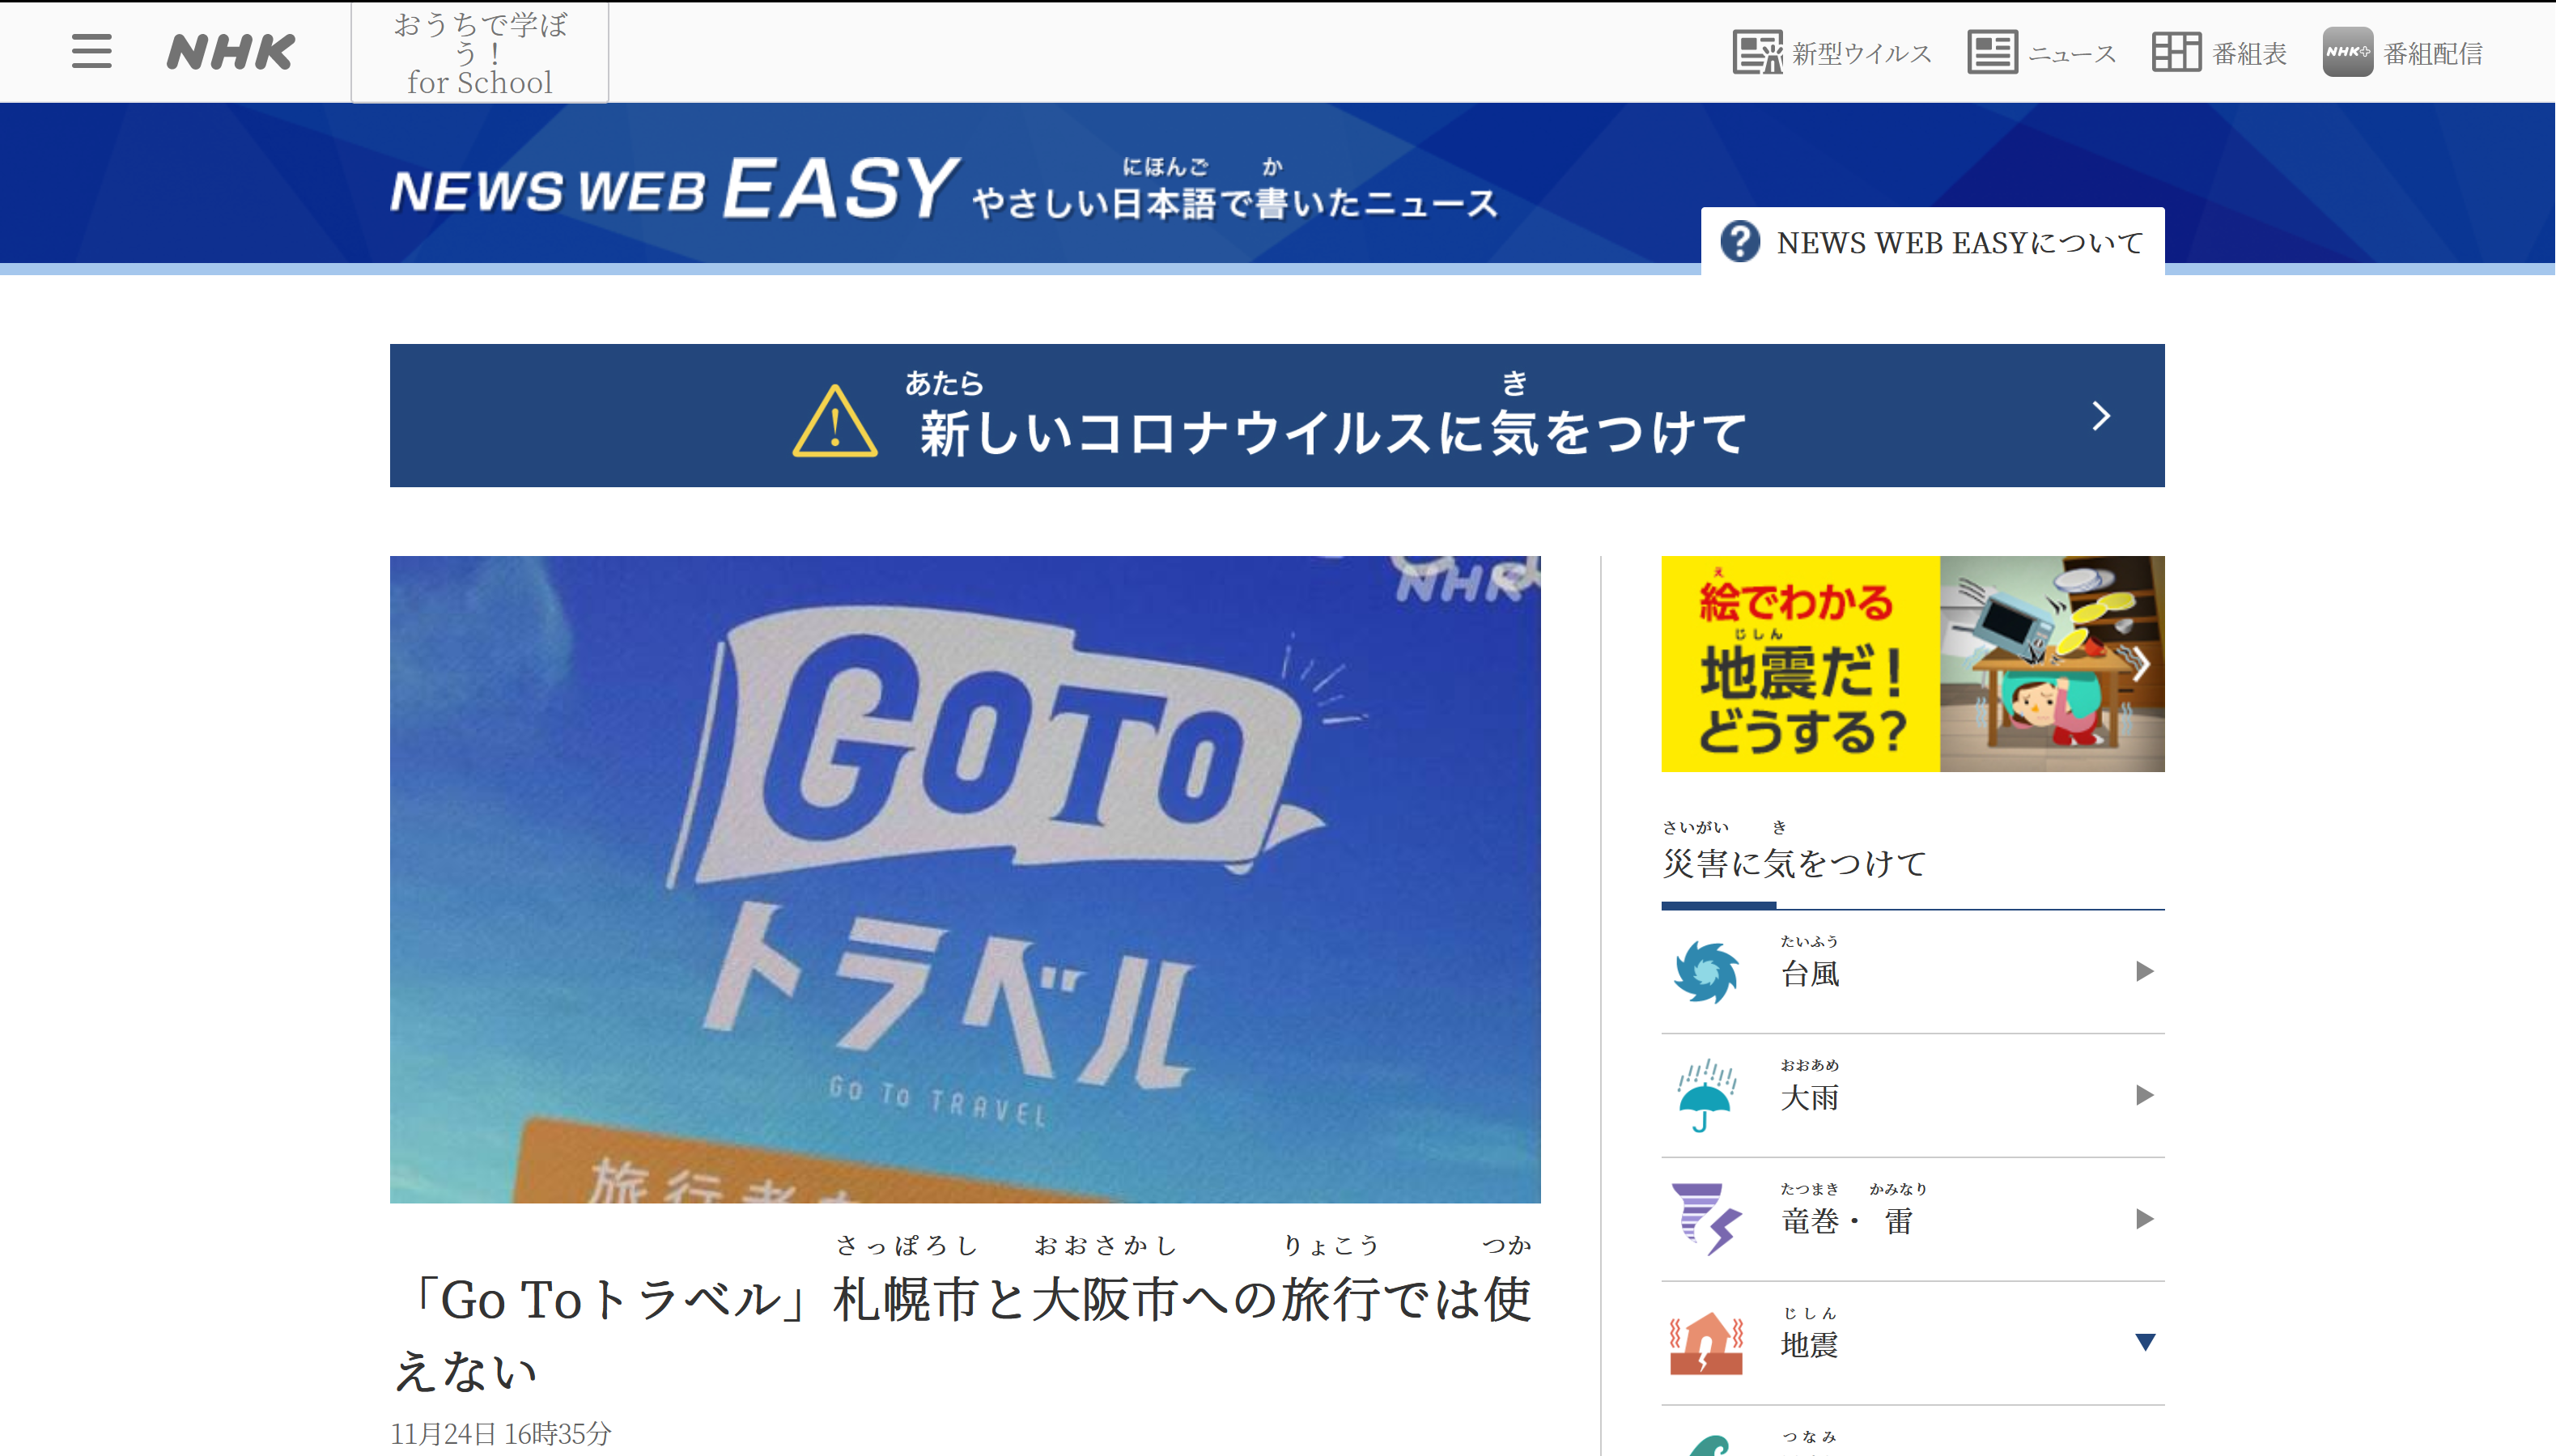
\includegraphics[width=\textwidth]{NHKniYoukoso.png}
  \caption{Главная страница News Web Easy}
  \label{NHK}
\end{figure}


%% ---------- subsection ---------- %%
\section{Текущее положение дел в системах упрощения текстов}
%% ---------- subsection ---------- %%


Вообще говоря, на сегодняшний пока ещё день не существует достаточно качественной системы упрощения текстов, способной заменить ручной перевод "--- дела здесь обстоят немногим лучше машинного перевода (из одного языка в другой), что можно объяснить отсутствием качественного и масштабного корпуса для обучения модели упрощения текстов (не только для японского языка, но даже для английского) и довольно высокой сложностью самой задачи, связанной с необходимостью «понимать» текст, что, к сожалению, современный искусственный интеллект сделать пока ещё не в состоянии.

Тем не менее, подобно тому, как сегодня используются системы машинного перевода (например, перевод отдельных слов или перевод текстов с последующими ручными корректировками), могут использоваться и системы упрощения текстов.


% .---|||___|||--- C H A P T E R ---|||___|||---. %
\chapter{Теоретическая часть работы}
% .---|||___|||--- C H A P T E R ---|||___|||---. %


% .---|||___|||--- S E C T I O N ---|||___|||---. %
\section{Этапы обработки естественного языка}
% .---|||___|||--- S E C T I O N ---|||___|||---. %


Как правило, в обработке текстов обычно выделяют следующие этапы~\cite[с.~9]{Batruha}:
\begin{enumerate}[1.]%
  \item Графематический анализ.
    Здесь осуществляется анализ на уровне символов, в том числе и токенизация, то есть разбиение набора символов (текста) на последовательность отдельных структурированных частей (слово, знак препинания, число, гиперссылка, адрес электронной почты и~т.\,д.).
  \item Морфологический анализ.
    Здесь происходит анализ на уровне слов (не токенов).
    Стоит выделить следующие процессы, проходящие на этом этапе:
    \begin{itemize}%
      \item Лемматизация
        "--- это нахождение нормальной (начальной) формы слова (леммы), к примеру, лемма у слова «сбегать» "--- «бегать».
        В японском это относится в основном к глаголам, так как у существительных, как правило, всего одна словоформа. 
      \item Приписывание граммем.
        Граммемы "--- грамматическая характеристика, например, род, падеж, число.
        Граммемы могут помочь в разрешении неоднозначностей, которые возникают в морфологии.
    \end{itemize}
  \item Фрагментационный анализ.
    Осуществляется на уровне фраз, частей предложений. Этот этап неразрывно связан с синтаксическим анализом, а иногда и вовсе говорят о них, как об одном целом. Сюда, например, может входить обработка причастных или деепричастных оборотов.
  \item Синтаксический анализ.
    Осуществляется на уровне предложений.
    Здесь, как правило, строится дерево зависимостей одних слов от других, а также исключается морфологическая неоднозначность.
  \item Семантический анализ.
    Осуществляется на уровне всего текста.
    Самый сложный и неоднозначный из этапов, здесь появляется формальное представление смысла текста, как правило, в виде сементического графа.
    На сегодняшний день задачи семантического анализа чаще всего решаются искусственными нейронными сетями, о чём мы и поговорим далее.
\end{enumerate}


% .---|||___|||--- S E C T I O N ---|||___|||---. %
\section{Искусственные нейронные сети}
% .---|||___|||--- S E C T I O N ---|||___|||---. %


Вкратце, искусственная нейронная сеть (ИНС) представляет собой систему соединённых и взаимодействующих между собой простых нейронов. Каждый нейрон получает на вход несколько чисел (входные данные или же выходы других нейронов), суммирует эти числа с определёнными коэффициентами (нахождение оптимальных коэффициентов "--- обучение ИНС), после чего применяет к сумме функцию активации (любую нелинейную функцию) и передаёт результат на вход другому нейрону (или же на выход ИНС).

Существует большое множество различных архитектур ИНС (свёрточные, рекуррентные, рекурсивные, графовые и~т.\,д.), однако в данной работе будет сконцентрировано внимание на так называемых трансформерах (Transformer), используемых, как правило, для языковой обработки, в частности для задач перевода и упрощения текстов.


% .---|||___|||--- S E C T I O N ---|||___|||---. %
\section{О модели Transformer}
% .---|||___|||--- S E C T I O N ---|||___|||---. %


Transformer "--- относительно новая (2017~г.) архитектура глубоких ИНС, разработанная в Google Brain.
Так же, как и рекуррентные ИНС (РНС), трансформеры предназначены для обработки последовательностей (к примеру, текста), то есть трансформеры относятся к sequence-to-sequence (seq2seq) моделям. В отличие от РНС, трансформеры не требуют обработки последовательностей по порядку, благодаря чему они распараллеливаются легче, чем РНС, и могут быстрее обучаться.

Используются трансформеры, например, в Яндексе (там его используют для лучшего ранжирования запросов, то есть поиск идёт не только по тексту, как обычной строке, но и по смыслу этого текста), во многих переводчиках (Яндекс, Google, DeepL и~т.\,д.), а также в GPT-3 "--- самой большой на сегодняшний день модели генерации текстов на английском языке.

% Нужно будет переписать {
% 
% 
% 
Трансформер состоит из кодировщика и декодировщика (encoder~\&~decoder). Кодировщик получает на вход последовательность слов в виде векторов (word2vec). Декодировщик получает на вход часть этой последовательности и выход кодировщика. Кодировщик и декодировщик состоят из слоев. Слои кодировщика последовательно передают результат следующему слою в качестве его входа. Слои декодировщика последовательно передают результат следующему слою вместе с результатом кодировщика в качестве его входа.

Каждый кодировщик состоит из механизма внимания (attention) (вход из предыдущего слоя) и ИНС с прямой связью (вход из механизма внимания). Каждый декодировщик состоит из механизма внимания (вход из предыдущего слоя), механизма внимания к результатам кодирования (вход из механизма внимания и кодировщика) и ИНС с прямой связью (вход из механизма внимания).

Каждый механизм внимания параметризован матрицами весов запросов $W_{Q}$, весов ключей $W_{K}$, весов значений $W_{V}$. Для вычисления внимания входного вектора $X$ к вектору $Y$, вычисляются вектора $Q=W_{Q}X$, $K=W_{K}X$, $V=W_{V}Y$. Эти вектора используются для вычисления результата внимания по формуле~\eqref{attentionEq}. 
\begin{equation}\label{attentionEq}%
  \operatorname{Attention}(Q, K, V) = \operatorname{softmax}\left(\frac{QK^T}{\sqrt{d_k}}\right) V.
\end{equation}
% 
% 
% 
% }


% .---|||___|||--- S E C T I O N ---|||___|||---. %
\section{Выбор инструментов}
% .---|||___|||--- S E C T I O N ---|||___|||---. %


Для обучения модели будет использоваться Python в связке с фреймворком для машинного обучения TensorFlow~\cite{Tensorflow}, предоставляющий широкие возможности для реализации нейронных сетей, в том числе, там присутствует поддержка ранее упомянутых трансформеров.
Для токенизации будет использоваться библиотека MeCab~\cite{MeCab}.

Система будет доступна в браузере в виде простого приложения, то есть модель будет обучена на Python, а пользоваться обученной моделью можно будет в любом современном браузере (пользователю ничего не нужно будет устанавливать).
Для реализации веб-приложения будет использоваться JavaScript с фреймворком Svelte, позволяющим создавать современные и быстрые SPA-приложения.
